\section{Empirical mechanism comparison}
\label{sec:expr-comparison}
In this section we compare the algorithms that we have presented in
terms of runtime performance and the satisfaction of the exact
proportion condition. For our comparison we use synthetic data that
capture different scenarios for the budget distribution across the
population. In all of the scenarios we assume that the prominence in
different rank positions follow the Zipfian distribution that we
observed in Section~\ref{sec:expr-odesk}.

\subsubsection{Runtime performance}
\label{sec:expr-runtime}

We compare the runtime performance of the EP algorithm
(Algorithm~\ref{alg:find-equitable}) and two different variations of
the RT algorithm (Algorithm~\ref{alg:tontine}). In the first
variation, called \emph{naive} RT, we renormalize the weights of
individuals after each assignment of an individual to a position. In
the second variation, called \emph{tree-based} RT, we leverage the
tree structure described in Section~\ref{sec:tontine}.

The comparison setting is the following. For different sizes $n$ of
the population we assign merit values to the individuals using uniform
sampling in the range $[0,1]$ and we set the prominence of each of the
$n$ search positions to follow a Zipfian distribution with exponent
$1.35$. We do not report results for other distributions in this
section, since our experiments showed that the distribution types have
negligible impact on the algorithms performance. For each value of $n$
we ran all of the three algorithms and we measured the runtime in
seconds. 
\begin{figure}[t]
  \centering
  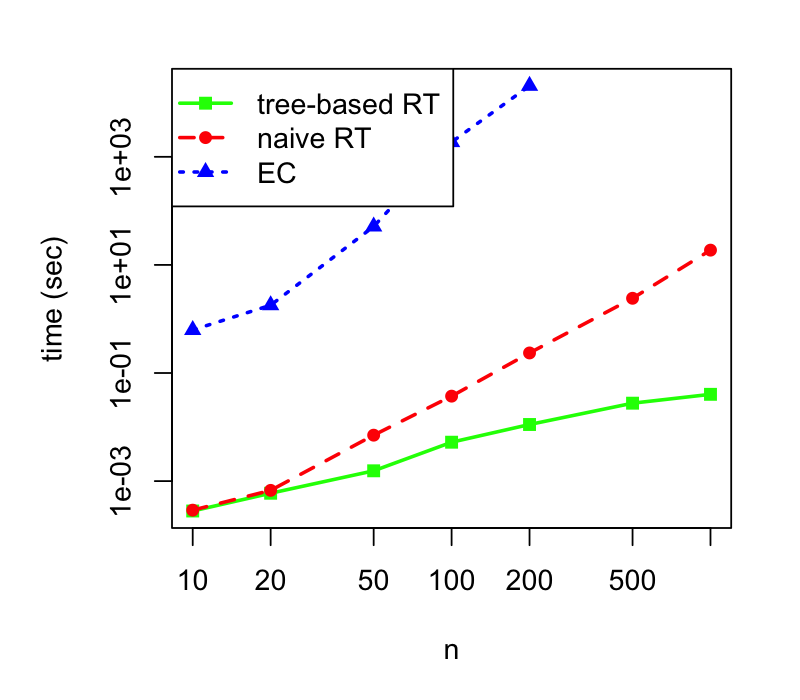
\includegraphics[width=0.6\columnwidth]{../simulations/results/performance.png}
  \caption{Runtime comparison of the three different assignment
    algorithms.}
  \label{fig:runtime}
\end{figure} 
We report the results in Figure~\ref{fig:runtime}. The x-axis shows
the number of individuals in the population and the y-axis shows the
time in logarithmic scale. There are three lines in the plot and each
line looks at a different algorithm. The solid line looks at the
tree-based RT, the dashed line looks at the naive RT, and the dotted
line looks at the EP algorithm. The closer a line to the x-axis the
better the algorithm. We observe that tree-based can rank up to $1000$
individuals in much less than a second. The tree-based RT achieves
also significantly faster runtime than the naive RT, which shows the
benefits of the tree structure we use to expedite sampling. As far as
the EP algorithm is concerned, we did not to run it for $n$ greater
than $200$, since the $6$ hours it took to rank $200$ individuals
convinced us that it cannot be used in practice. To summarize, the
tree-based RT algorithm is much faster than the other algorithms and
its runtime make it practical for real-world scenarios.


\subsubsection{Equitable prominence approximation}
\label{sec:expr-approximation}
Although we showed that the RT algorithm is fast enough to be applied
to real-world scenarios, we have not still evaluated its impact on the
prominence allocation problem. Recall that the algorithm does not
yield equitable prominence in the general case as the EP algorithm
does. However, the RT algorithm ensures continuity and monotonicity in
merit, two properties that are missing from the vanilla assortative
ranking.

In this section we compare the assortative ranking, and the rankings
obtained from the RT and the EP algorithms in terms of their
prominence allocation for different merit distributions. To obtain
different merit distribution we sample from the Pareto distribution
with different $\alpha$ parameters. Recall that when $\alpha$ is
large, the Pareto distribution approaches the Dirac distribution at
point $1$. That means, that all of the sampled individuals' merits
will be almost equal to $1$. As the value of parameter $\alpha$
decreases, the merit values get spreaded out and finally the Pareto
distribution becomes skewed. That is, it yields few individuals with
extremely high merit values and many individuals with low merit
values. To evaluate the effect of the different rankings across the
spectrum of different Pareto distributions we used the following
values for $\alpha$: $100$, $10$, $5$, $1$ and $0.5$. Although
we use different merit distributions,we use in every case a Zipfian
distribution with exponent $1.35$ to model the prominence distribution
over the search positions.

For each distribution of merits we ran each of the algorithms $m$
times to obtain the average prominence for each individual $\bar{v_i}$
across the $m$ runs\footnote{We did not actually run the EP algorithm,
  since it was theoretically shown to achieve equitable prominence
  allocation}. To evaluate the success of the algorithms in achieving
equitable prominence allocation, we use the root mean square error
(RMSE) defined as:
\[
\sqrt{\frac{\sum_{i=1}^n\left(\frac{b_i}{\sum_{j=1}^n
        b_j}-\frac{\bar{v_i}}{\sum_{j=1}^n \bar{v_j}}\right)^2}{n}}
\]
\begin{figure}[t]
  \centering
  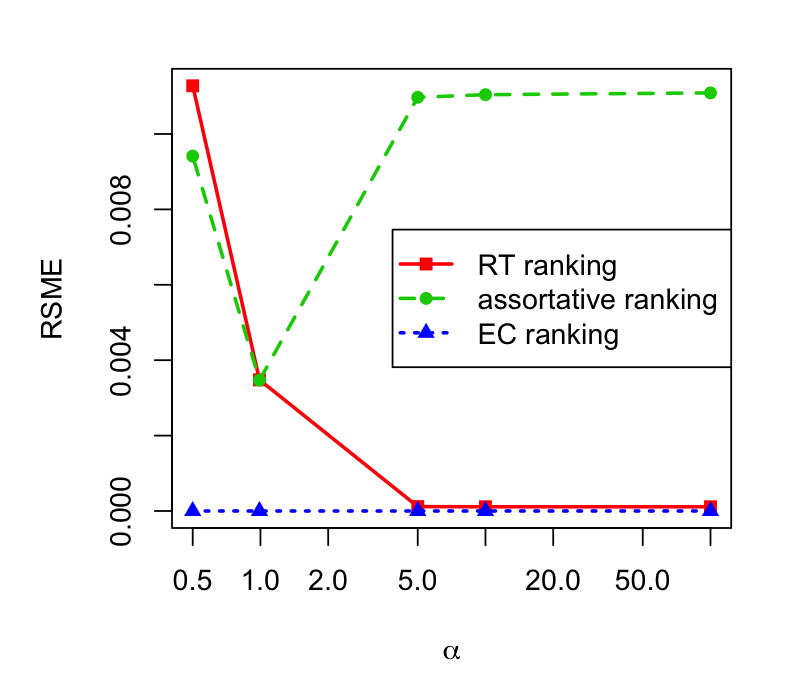
\includegraphics[width=0.6\columnwidth]{../simulations/results/approximation.png}
  \caption{RMSE in the approximation of equitable allocation for the
    three different ranking approaches. The contractor merits are
    randomly sampled from a Pareto distribution with parameter $\alpha$.}
  \label{fig:approximation}
\end{figure} 
We plot the results in Figure~\ref{fig:approximation} for
$m=1000$. The x-axis shows the value of the Pareto distribution
parameter and the y-axis shows the RSME. There are three lines in the
plot and each looks at a different ranking approach. The solid line
looks at the RT ranking, the dashed line looks at the assortative
ranking and the dotted line looks at the estimated EP ranking. Note
that RMSE is 0 for the EP ranking, since the EP algorithm is
guaranteed to achieve equitable prominence allocation for any merit
distribution. The assortative distribution has small RMSE for low
values of $\alpha$, because in these case the merit distribution
become similar to the Zipfian prominence distribution. However, the
real-world data in Section~\ref{sec:expr-odesk} showed that these
distributions are not similar. As $\alpha$ increases the assortative
ranking yields significantly greater RMSE that the other ranking
approaches. Finally, note that the RT ranking yields RMSE that is very
close to $0$ for a wide range of $\alpha$ values. The RMSE increases
for small values of $\alpha$ that yield distributions that were not
observed in the oDesk dataset. Thus, we can conclude that the RT
algorithm yields prominence that is close to the equitable allocation
for practical cases. This result combined with its ability to scale
make it an attractive option for real-world applications.


